\documentclass{article}
\usepackage{graphicx}
\usepackage{listings}

\begin{document}
\lstset{language=SQL, tabsize=3, basicstyle=\footnotesize, columns=fullflexible, breaklines=true}

\title{Database for EIOtraining}
\author{Oliver-Matis Lill}
\maketitle


My goal is to make a database for all the functionality in the EIOtraining website. The database needs to store the data of the EIOtraining users, the news and the problemset entries. It's users will be mainly problem creators who create programming problems, and students who solve them. This database is necessary for the EIOtraining website to work, because users, news and prolemset entries need to be stored somewhere.

The database class model looks like this:
\begin{center}
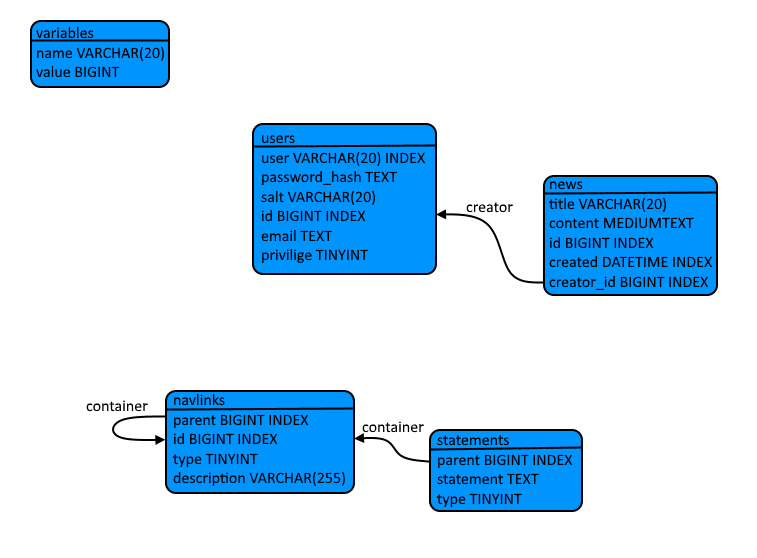
\includegraphics[scale=0.65]{database.png}
\end{center}

I used "paint.net" to draw this model. The usage of entities should be self explainatory. "users" contains the account data for each user, "news" contains the news with a reference to the user that created it. "variables" are simply some presistent variables used in EIOtraining. "navlinks" is the least obvious, each navlink is basically a folder, that contains other navlinks or a statement, depending on type. "statements" simply contains the problem/tutorial statements.

The SQL statements to create this relational database are:
\lstinputlisting[frame=single]{create.sql}
And the "users" table in it looks like this:
\begin{center}
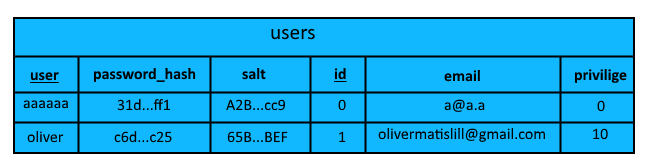
\includegraphics[scale=0.65]{rel.png}
\end{center}

This table is obviously not in third normal form, because all this data is needed for every user anyways. Using a single table makes database smaller by avoiding duplicate attributes and indices and also makes queries much simpler. The normal form of this table would look like this:

\begin{center}
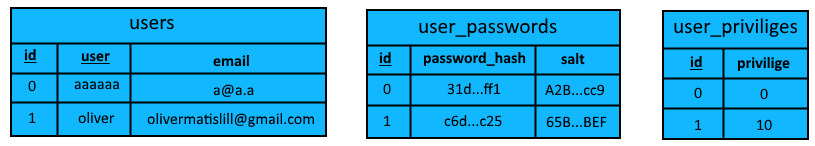
\includegraphics[scale=0.65]{normal.png}
\end{center}

The database has been realized in the EIOtraining website using MySQL.

This procedure signs up an user:
\lstinputlisting[frame=single]{proc1.sql}

The output was:
\lstinputlisting[frame=single]{proc1out.sql}

This procedure retrieves the data of a news story and it's creator user:
\lstinputlisting[frame=single]{proc2.sql}

The output was:
\lstinputlisting[frame=single]{proc2out.sql}

This procedure updates a statement:
\lstinputlisting[frame=single]{proc3.sql}

The output was:
\lstinputlisting[frame=single]{proc3out.sql}

This procedure retrieves a statement by it's navlink description>
\lstinputlisting[frame=single]{proc4.sql}

The output was:
\lstinputlisting[frame=single]{proc4out.sql}

This procedure retrieves all navlinks and their statements, if present:
\lstinputlisting[frame=single]{proc5.sql}

The output was:
\lstinputlisting[frame=single]{proc5out.sql}



\end{document}